%\chapter{Background}
%%labels will help you to reference to certain images, tables, chapters, section, and so on...
%\label{background}


\chapter{Background and Related Work}
\label{relatedWork} 





%DELETEME: This chapter will cover all of your background information and related work. Background and related work are directly related to your thesis. Please do not place irrelevant content here which is a common mistake. Citing will be handled in the appendices.

%\todo{check the label with the old and new texts after restructure}


%In this chapter we discuss Amazon's state-of-the-art strategy
%%before moving on to related work in other archetypes 
%as it is important to introduce the implementation scope of voice assistants 
%top down
%%bottom-up 
%prior to exploring the current context 
%%within the same boundaries of voice assistants 
%%then 
%after comparing it to other approaches in the larger context of conversational bots as a whole from a technical and user experience point of view. 


%moved to gui section
%We start with a juxtaposition of Voice User Interface (VUI) to the Graphical User interface (GUI) respective to cognition and behavioural design which gets us to define new terminological foundation that will follow throughout this thesis.

%moved to chapter 3: to then elaborate on implementation requirements in Section \ref{frameworks_structs}. 


%DELETEME: Background represents underlying knowledge that is required to understand your work. The expected knowledge level of your readers can be set to the one of a bachelor or master student who just finished his studies (depending on what kind of thesis you are writing). This means that you do not need to describe how computers work, unless your thesis topic is about this. Everything that an avarage alumni from your field of studies should know does not need to be described. It turn, background information that is very complex and content-wise very near to you problem, can be placed in the main parts. Everyting else should be written here. Note: it is important to connect each presented topic to your thesis. E.g. if you present the ISO/OSI layer model you should also write that this is needed to understand the protocols you plan to develop in the main parts.







%#############################################################################
%###################### Related work (Bkgrd) ########################################
%#############################################################################

%DELETEME: Related work respresents results from work that handled the same or a similar problem that you are addressing. This work might have used a different approach or might not have been that successful. Finding a paper / work that solved your problem in the same way you were planning to do is not good and you should contact your supervizor for solving this issue. Again, each paper / work has to be connected to your approach: other papers might have not chosen an optimal solution; they might not have been taking care of essential aspects; they might have chosen a different approach and you believe, yours will work better ...

%\chapter{Related Work}
%\label{relatedWork}

As our motivation stems from the unstoppable worldwide trends of digitalisation, in this chapter we discuss current application categories
with respect to chatbots and voice assistans
and talk about governments' efforts in keeping up with these trends as part of their 
modernisation stream
%technology streams 
%in governments 
in the age of social media, Internet of Things (IoT) and the interaction between both.
We then show relevant examples in our context of voice assistants.




\section{Topology of Chatbots and Voice Assistants}

%ubiquity of voice, searchmetrics report
Chatbots and voice assistants come in numerous mouldings; on the web, in apps, through smartphones or as a combination of those and beyond. In Barot and Oren \cite{guidetochat} we observe the different purposes the industry caters for. As we witness the integration of chatbots in retail, productivity, entertainment and create more possibilities to integrate them in our daily lives, it is obvious that the trend will continue for a while before the market is saturated. Similar to marketplaces for applications like Apple's App Store and the Google Play Store which have become a commonplace term even though their slow stagnation in the recent years, chatbots and voice assistants are predicted to remain trendy until at least 2020 as per VoiceLabs figures %(Figure \ref{voiceLabs:mktpreds}).
\todo{es gibt tausende von möglichen statistiken, die man hier einbinden kann. Sind Worte trotzdem genug Beschreibung?\\
%\ref{voiceLabs:mktpreds} do
%Google Actions graph (call mom) w ezzay makonnash met3awedin w ba2ena now (statistic use at home more than outdoors etc)
}
Moreover, SearchMetrics' upcoming report has a section dedicated to voice searches as the analyst company advises on SEO tweaks for Google Voice Search \cite{searchmetrics:blog} and argue how voice assistants are becoming a ubiquitous market.


\todo{%move / remove what is irrelevant
	%	In this section, we conduct a short survey of problems we can face with natural language
	
	
	\textbf{by category}\\
	- leisure /
	- \href{https://www.forbes.com/sites/tomaslaurinavicius/2017/04/24/facebook-messenger-bots/\#4f61c16a66d8}{fun bots}  / 
	- productivity / 
	- more (graph from voicelabs report) \\
	- what are classic use cases for their use with prominent examples?\\ Booking tickets (e.g. airline bot)\\ %KLM
	- quick survey of respective 'AppStores'\\
	\textbf{by purpose}\\
	-physical locations (home, office, car, phone, in a business)\\
	Information bots\\
	\textcolor{magenta}{
		- mention available service types (information system as a "webpage/DB")\\
		- vs an interactive bot that gives you customized information on demand\\
		- hier soll der D115 Anwendungsfall "Beauskunftung" kurz erl\"autert werden\\
	}
	social bots (not a focus)\\
	\textcolor{magenta}{
		- with advantages / disadvantages\\
		- fake news / online reviews\\
	}
	more on AI in bots (optional)\\
	\textcolor{magenta}{
		- use of ML\\
		Handyversicherungsbeispiel\\
		- from business perspective, the bot is aiming to sell more polices,\\ 
		- the bot tries to determine if there is a nuance in the user's answer (machine acting as a judge!)
		- e.g. ``how did the phone fall off``
		- MKTG - Aufwand
	}\\
	IFTTT Applets for voice commands\\
	IFTTT didn't work because it was semi automated. you needed to zwischgreifen (Ivo Lehrter)
}











%###################################################################################
%###################### E-GOVs           ########################################
%###################################################################################

\section{Digitalisation in the Public Sector}

There is no doubt that social media has changed the shape of our society in the last twelve years. Not only by affecting the way we communicate, but also by generating immense amounts of data, creating new jobs and disrupting economies en masse.
Meanwhile, governments are continuously striving to market their image in more creative ways than ever to target more segments in society. From what used to be a novelty, politicians' tweets are now a highlight in main news sections. The sudden interest of governments in social media platforms 
can be seen as an attempt to become more transparent and reach more public awareness. It is more likely for instance that a 15-year old would find out about a public figure (including a president) by following their story on Instagram than by reading news about them on dedicated news website.

This is ultimately because the social media platform, as part of many new technologies are designed with the focus of reach in mind much more than only availing information to the target.
We distinguish between the pull-based model of information retrieval, where a person would actively look for certain information usually through looking something up, vs. the push model, where the information is `thrown' to the user without them actively asking for it, usually by subscribing to the source or news outlet and more likely through audiovisuals than trough text. Unsurprisingly, such platforms become a key player in redefining fame, identity and image.

The push-model is a new strategy to dissemination of knowledge, which governments %also decided to 
embrace \cite{forbes:govOutreach} to bridge the gap in their outreach to the public. 
Although the digitalisation trend in governments generally emerges from the desire to expand infrastructure for information exchange and availing open government data \cite{un:egovReport}, digital media has now become an integral part of it, too, making it inseparable from many institutions compositions. 

In Germany, many advanced milestones in digitalisation were attained in the last years. From eliminating paper in many administrative workflows 
%in government bodies %sssssssssss
to funding successful start-ups in the field (e.g.Aaron.ai \cite{exist:aaron})
and seeking renewable energy as a foundation %of scale 
to power an exponentially growing number of devices in the country with a reduced carbon footprint, the aspect of digital media has been relatively neglected compared to other countries.
According to numbers from the United Nations' E-Government Development Index in 2016, Germany ranked 15th worldwide and 8th within Europe with an average of 0.82 % of its services provided or operated digitally 
, substantially outranked by the United Kingdom, the United States, Singapore and France. Outperforming its previous statistics from 2014 where its index scored  0.79 with a world average of 0.47, where it was also outranked by Austria, Israel and Bahrain \cite{freiheit:digitalisierung} in addition to the aforementioned countries as listed in Figure \ref{un:egci}.  Germany's ranking went up from 21st to 16th worldwide in the last two years.

\begin{figure}[h]
	\caption[E-Government Development Index in Europe]{Top Ten Countries for E-Government Development Index in Europe based on \cite{un:egovReport}}
	\label{un:egci}
	\includegraphics[width=\textwidth]{Govcharts/TopTenEUeGov} 
\end{figure}


the E-Government Development index (EGDI) is composed of a calculation based on proportionally normalised averages of the Online Service Index (OSI), the Human Capital Index and the Telecomunication Infrastructure Index. 
%as can be seen from Figure
When it comes to engagement through e-participation, Germany performance lies also in the top quartile. Its Online Service Index performed 21st worldwide (Figure \ref{un:osi}), which shows the continuous strive to maintain relatively many rights to access government information online and an open data government policy on the web.

\begin{figure}[h]
	\caption[United Nations Online Service Index (Top 30)]{Online Service Index for Top 30 Countries Worldwide based on The UN Department of Economic and Social Affairs \cite{un:egovReport}}
	\label{un:osi}
	\includegraphics[width=\textwidth]{Govcharts/osicopy} 
\end{figure}

In an age where we
take the internet for granted,
we also expect to have multiple communication channels open to government representatives and public authorities. 
%just like we 
%it for granted to be able to check flight delays on a designated platform, we also expect to constantly have immediate access to a communication channel with local and global representatives.
%
%Governments targets in social media have become  digitalisation 
%it started with social media-now want to give a face and experience(kan2oho sherka) not only by eliminating paper 
% eliminating carbon footprint. almania w heya gamda keda w bte3mel atomkraft nein danke
%\todo{bring up the Freiheit.org chart \cite{freiheit:digitalisierung}\\ 
%	Talk about digitalisation in general (how there are talks in DE about autonomous driving and the related regulations - ref Haase)\\
%	say that \\ bass}
Hence, out of public interest, governments are advised not only to focus on digitising their internal structure, but also their representation on the public sphere.
Especially at times of change like with the introduction of autonomous driving and the regulations related to it, transparency is a continuous expectation from the people. As stated above, since transparency heavily relies on public presence, which in turn depends on availing more communication platforms, voice assistant services are definitely worthy of consideration in that context.




\section{Worldwide Examples of Bots in E-Government}

Knowing that the Online Service Index of a country consists of the services available to different groups of society, we can argue that 
%it is also important to acknowledge how 
vulnerable groups (i.e. the poor, persons with disabilities, older persons, immogrants, women and youth) can be easily marginalised in this index. Another statistic by the German Federal Statistics Office (Statistisches Bundesamt) shows that most online public services in 2016 were targeting persons of age 25-44 with an equal offer of services for age groups 45-67 and 16-24 with the least amount of services targeted at youngsters between age 10 and 15 comprising 15\% of the service catalogue (Leistungskatalog, LeiKa) \cite{stabunda:leika}.
For that reason, we acknowledge the importance of inclusion especially towards vulnerable groups in the process of expanding a online public service.

This gives us the advantage to promote in the development process of a chatbot or a voice service assistant for inclusion especially since the domain is relatively still uncharted. As Zehlike et al. conclude, given the many possible biases Machine Learning Algorithms can result in \cite{fa:ir}, a holistic approach is required to have a balanced distribution of services in different fields (e.g. Health, Finance, Administration) for different groups of society (protected and unprotected groups).
%(children, elderly, foreigners, locals, immigrants, men, women, youth).
Already offering a service on platform that offers less constrains to the user than a browser's graphical user interface (GUI) allows per se more options for inclusion but could also be limiting of the system reacts to a vocabulary used only by a certain group for instance.

In terms of functionality and testing of a chatbot or voice assistant system on inclusion metrics, WitLingo \footnote{\url{https://www.witlingo.com/}}, a company which builds voice-driven apps for banks, universities, law firms as well as other public and private sector enterprises believes in that sense that ``getting feedback [on the performance of the voice service to different groups of people] is more important than measuring ROI'' \cite{witlingo:bouzid} with a report that reflects the same statement in the retail sector from Voysis and Retail TouchPoints \cite{voysis:report}.


%sssssss

%\todo{
%%	WitLingo: which builds voice-driven apps of all sorts for banks, universities, law firms, and others.\\
%%	aaron.ai use cases (local examples)\\
%%	
%%	\textbf{eingehen auf} Singapore / LA /.. as cities that have a higher index of e-gov and use chatbots\\
%
%%	say you chose wienbot and askgeorgia as german and english counterparts
%}


	While there are several cities such as Singapore and Los Angeles integrating chatbots and voice assistants into their administration's websites and coming up with all sorts of interactive solutions,
	for this research we choose the City of Vienna chatbot service \href{https://www.wien.gv.at/bot/}{\textsc{WienBot}\footnote{\url{https://www.wien.gv.at/bot/}}} given that it uses German 
	and the Alexa Skill \href{https://www.amazon.com/GeorgiaGov-Interactive-GTA-Ask/dp/B074XBQGTQ}{\textsc{GeorgiaGov}}\footnote{\url{https://www.amazon.com/GeorgiaGov-Interactive-GTA-Ask/dp/B074XBQGTQ}} for a comparison in US English, as we examine both languages in our development process.

\subsection*{\textsc{WienBot}}
Started out of an amateur project and officially launched in December 2017, the chatbot is developed for Vienna, Austria by \inote{waiting for answer from Sindre Wimberger..}
this was the first official chatbot made for a city council. 
\todo{pics of interface and conversation\\
	the idea of `stories'\\
mention what aspects of the model we can mock. e.g. their \@wienbot twitter feed re new launches.
\url{https://futurezone.at/digital-life/wienbot-die-stadt-wien-hat-einen-chatbot/246.709.043}}




%\todo{
%	\\
%	Ask GeorgiaGov is developed by that company (get source)
%}
\subsection*{\textsc{GeorgiaGov}}
developed for Georgia, USA by Acquia\footnote{\url{https://www.acquia.com}} ...
\todo{pics of conversation}

\begin{quotation}
The state of Georgia has always been on the forefront of web accessibility. For example, from 2002 until 2006, Georgia piloted a time-limited text-to-speech telephony service which would allow website information and popular services like driver's license renewal to be offered to citizens \cite{dries:georgia}
\end{quotation} 


	While we are less interested in the content delivered through the voice assistant and have no access to AskGeorgia from the German Amazon Store, we use the US store for our conversation testing purpose to pick the relevant design of flow of conversation. %tab3an di f amrika fal mawdou3 mokhtalef, bas el fekra here is el design not the exact content

















%###################################################################################
%###################### Use Case in detail  ########################################
%###################################################################################
\section{Berlin as a Use Case}
\label{blnusecase}
As Schwarzer et al. state, few systems are available that ``enable Berlin’s citizens to get informed about governmental services'' \cite{lomm:gov}.
As part of the modernisation process, the \textsc{Virtual Citizen Assistant (Virtueller Bürgerassistent)} was born in \inote{developed by?} 
the Information Retrieval and Machine Learning Competence Centre of the Technical University of Berlin's Distributed Artificial Intelligence Laboratory.



\todo{-\textbf{Theorie}\\
	-summarize LeiKA infobroschuere(BMI08324screenBarrierefrei.pdf)\\
	-Welche Daten gibt es?\\	  
	-Was sind die Erwartungen?\\ 	
}


\todo{
	\textbf{current berlin.de bot}\\
	- dienstleistungen.json structure (finding the info through hierarchical nodes)\\
	- interpreting the nodes as intents\\
	- traversing the nodes (one level up then to next node)\\
	- no session/no persistence\\
	- explain how the json nodes map to intents and cores in solr etc
	
	%x	x	x
	%ooo ooo ooo
	%try first, go to second (kosten, zeit, rechtsgrundlage, ..) skip one if it has already been suggested.. hinweis..that is built into the xml
	%
	%the live service is different than the one at DAI
	
	- developed as a webapp using groovy.\\
	- what to mention about AllInclusive?
	- whatever it is, it should go here or before it can go in implementation section.\\
	- structure of Hitlist on berlin.de  is provided by ITDZ \\
	- explain LeiKa old and new JSON as an intro to API\\
}



We cover here an excerpt of basic elements that we will later see more or less in the same structure of the JSON file containing the interaction model:\\




\todo {change this into a table and add a tree list like the interaction model in appendix}

\begin{table}[htbp]
	\caption{relevant nodes in query results \mintinline{java}{Dienstleistungen.json} - Description}
	\label{dienstleistung:descr}
	\begin{tabu} to \textwidth{|X|X|X|X[2]|}
		key & type & ex. Value & description\\ \hline \hline
		
		\lstinline|id| & \lstinline|int| & 326233 & public service ID % on \href{https://service.berlin.de}{service.berlin.de} 
		\\
		
		\lstinline|d115URL| & %URL 
		\lstinline|string| & %''https://service.berlin.de/dienstleistung/326233/'' 
		& link to public service URL % on  \href{https://service.berlin.de}{service.berlin.de} 
		\\
		
		\lstinline|d115Name| & \lstinline|string| &  FxionsB. % Fiktionsbescheinigung 
		& public service name %as listed on \href{https://service.berlin.de}{service.berlin.de/dienstleistungen} 
		\\		
		
		\lstinline|ssdsAll| & \lstinline|string| & ... & \shortstack[l]{additional captive search terms,\\ synonyms used by Virtueller \\ Bürgerassistent. Found to be \\ helpful in conversations \\ with the chatbot} \\		
		
		\lstinline|d115Description| & \lstinline|string| & ... & \shortstack[l]{Introductory paragraph from \\the service web page \\ 
		Includes HTML tags}
		\\ %like <\backslash br> and <ul ...> \\		
		
		
		%		
		%		\mintinline{json}{d115Synonym} & \mintinline{json}{string} & ... & captive search terms, synonyms created by Virtueller Bürgerassistent \\		
		%		
		%		\mintinline{json}{d115Position} & \mintinline{json}{string} & ... & captive search terms, synonyms used by Virtueller Bürgerassistent \\		
		%		
		%		\mintinline{json}{d115InfoLaw} & \mintinline{json}{string} & ... & Legal base for offering this public service \\		
		%		
		%		\mintinline{json}{ssdsAll} & \mintinline{json}{string} & ... & captive search terms, synonyms used by Virtueller Bürgerassistent \\		
		%		
		%		\mintinline{json}{ssdsAll} & \mintinline{json}{string} & ... & captive search terms, synonyms used by Virtueller Bürgerassistent \\		
		%		
		%		
		%		
		%		
		%		
		%		
		%		
		%		\mintinline{java}{string} & \mintinline{java}{responsibility}  & denoting in which city halls a service is available\\
		%		\mintinline{java}{boolean} & \mintinline{java}{responsibility_all} & a flag set to true in case the service is available in all local authority offices / service points\\
		%		
		%%	\mintinline{java}{HTML list string} & \mintinline{java}{ description} &  not unified and includes text \\
		%%%		\item  \lstinline|<string> not unified and might need to have an \lstinline|int| added to it and set to 0 in case service is free
		%		\mintinline{java}{int} & \mintinline{java}{residence} & \\
		%		\mintinline{java}{int} & \mintinline{java}{id} & \\
		%		x & \mintinline{java}{representation}  & x\\
		%		\mintinline{java}{long} & \mintinline{java}{leika}  & \\
		%		\mintinline{java}{string} & \mintinline{java}{process_time}  &  need to derive minimum, average and maximum service times instead of a string, as well as conditions\\
		%		\mintinline{java}{string} & \mintinline{java}{name} & the name of the service that would make sense to a human \\
		%		\mintinline{java}{node} & \mintinline{java}{appointment}  &  \\ 		
		%%		% then inner node 
		%%%		\begin{itemize}
		%%%			\item \lstinline|link| (Key value with URL to /terminveinbarung page) - check if orphan or if it is for each beh\"orde and in that case how it gets the right one
		%%%		\end{itemize}	 
		%		\mintinline{java}{node} & \mintinline{java}{locations}  & \\ 
		%%		% then inner node
		%%%
		%%			\mintinline{java}{hint}
		%			\mintinline{java}{int} & \mintinline{java}{sth} & location| one of the 12 authorities \\
		%%%			\item \lstinline|url| of that service at that authority
		%			\mintinline{java}{node} & \mintinline{java}{appointment} & (a second one)	 \\	
		%		\mintinline{java}{node} & \mintinline{java}{onlineprocessing}  & \\
		%		\mintinline{java}{node} & \mintinline{java}{prerequisites} & \\
		%		\mintinline{java}{node} & \mintinline{java}{links} & \\
		%		\mintinline{java}{node} & \mintinline{java}{relation}  & \\
		%		\mintinline{java}{node} & \mintinline{java}{legal}  & \\
		%		\mintinline{java}{node} & \mintinline{java}{requirements}  & \\
		%		\mintinline{java}{node} & \mintinline{java}{forms}  & \\
		%		\mintinline{java}{node} & \mintinline{java}{authorities}  & \\
		%		\mintinline{java}{node} & \mintinline{java}{meta}  & \\
	\end{tabu}
\end{table}


%%%%%%%%%%%%%%%%%%%%
%provided in JSON for value lookup, the structure of the file is as follows: there are \inote{carry on - the structure}


%%%%%%%%%%%%%%%%%%%%%

%\Tree [.Dienstleistungen.json created [.VP [.V is ] NP ] ]
%
%\Tree[.Dienstleistungen.json 	
%	[.NP [.Det \textit{the} ]
%		[.N\1 [.N \textit{package} ]]]
%	[.I\1 [.I \textsc{3sg.Pres} ]
%		[.VP [.V\1 [.V \textit{is} ]
%			 	   [.AP [.Deg \textit{really} ]
%				  		[.A\1 [.A \textit{simple} ]
%							  \qroof{\textit{to use}}.CP ]]]]]]]




\todo{
	\textbf{API analysis}
	- missing variables e.g. are required papers, \\
	- flag: persönliche Vorsprache ja nein, ...\\
	- started with 616 Intents %in \lstinline|data| node 
	(now 685 or so), each containing \inote{Tableau}\\
	- should I include the JSON samples from Appendix here? or just refer to them?}
















\begin{figure}[h!]
	\caption{\mintinline{java}{Dienstleistungen.json}  - Primary Nodes}
	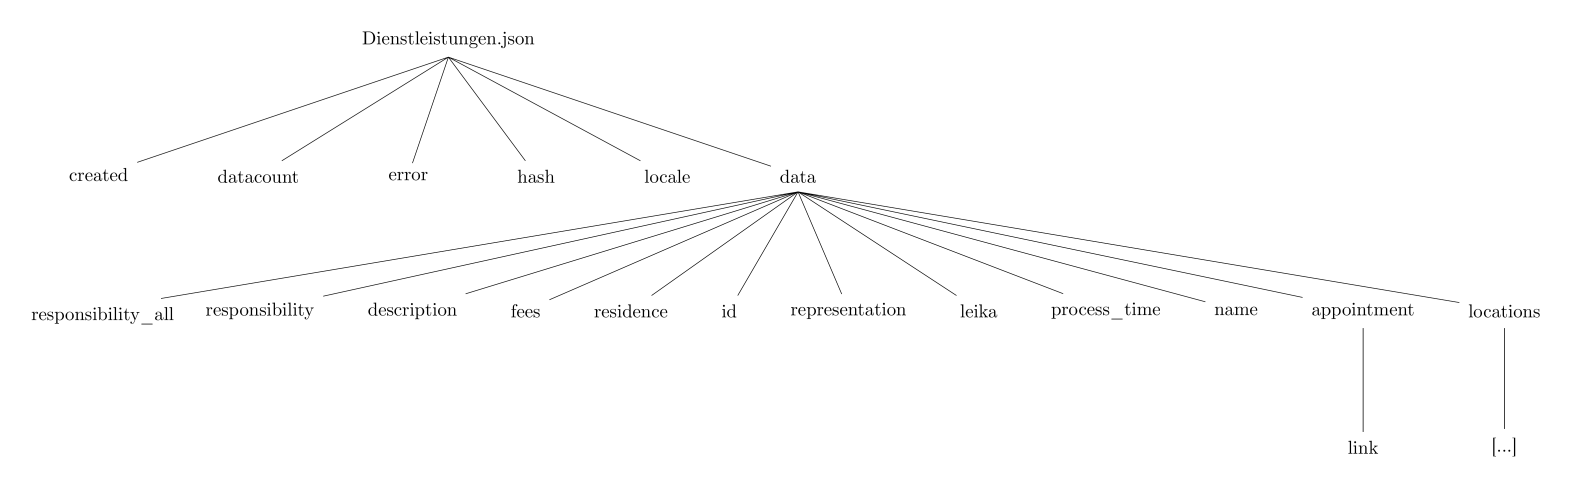
\includegraphics[width=\textwidth]{DLprim}
\end{figure}

\begin{figure}[h]
	\caption{\mintinline{java}{Dienstleistungen.json} - secondary Nodes}
	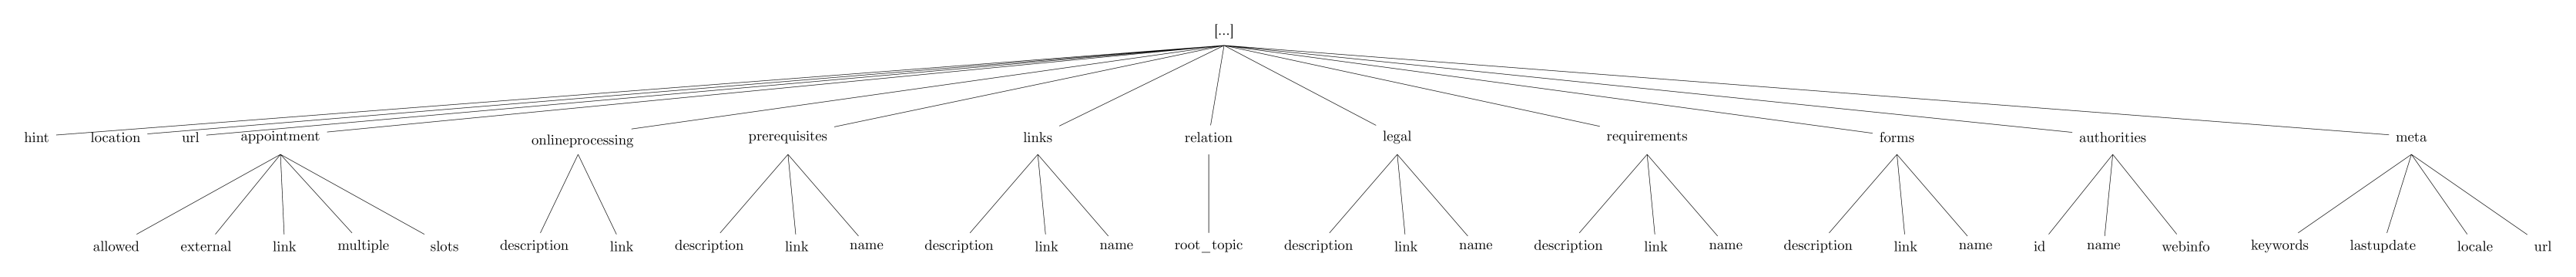
\includegraphics[width=\textwidth]{DLsec}
\end{figure}






\todo{\textbf{summary and ausblick}\\
	- static system as the Dienstleistungen do not change regularly\\
	-  as opposed to Versicherungsfirma z.B (ML tries to detect irregular patterns in case customer is lying).
	- unfortunately forums vs. FAQs did not work. if i want assistance, i want the customer to tell me the model number - and forums have mostly Schrott!\\
	- what the bot curently achieved is at least not give wrong answers, sometimes says idk but it doesnt confuse u. %same attitude like in lmny shops 
	- we talked about this in intro chapter. see if u want to mention again with a diff angle\\
	-(nur unpassende antworten sind frustrierend!)\\
}





%\subsection*{D115 and The Currently Deployed ``Virtual Bürgerassistent''}
%\todo{
%	- LeiKa

%	-Use case im Detail\\
%	- wie kann man die G\"ute des Systems beurteilen? \textbf{do not forget the surveyu made}\\   
%	- Meist sollte man in diesem Kapitel die L\"osung schon im Auge haben, um die Erwartungen so zu formulieren, dass die L\"osung auch geeignet ist?\\ 
%}























%###################################################################################
%###################### GUI/VUI ####################################
%###################################################################################

\chapter{The Voice as a User Interface} 
\label{vui}


We start with a juxtaposition of Voice User Interface (VUI) to the Graphical User interface (GUI) respective to cognition and behavioural design which gets us to define new terminological foundation that will follow throughout this thesis.

\section{GUI vs. VUI}
\label{guivsvui}

Visuals and Sounds can both communicate the same message even though they use a  completely different medium. One one hand, the premise that ``a picture is worth a thousand words'' can be valid based on the image but only assumes that we want to give a clear picture to the receiver. Communication through voice, on the other hand, can generally allow more room for interpretation. We think of an example where you would watch a football game on TV vs. the same game on radio, where listening to it allows each person in the audience group to imagine a different game for themselves, even though the match result are the same.


%%%Image

When we use written text, be it in a document or a street sign, or any label, we seek to mostly assure that all receivers understand the same message with a universal codification of what we want to express through the language we use. In this process, language becomes the common denominator for understanding and the short written text becomes purposefully designed to give in the best case a message not open to interpretation and so a foundation for an agreement or contract between the source and the destination of the message. It is a good medium of reference. 

%%%%%%%%%%%%%%%%%%%%%%%%%%%%%%%%%%%%%%%%%%
%voice message in airport - you can do your activity unobstructed
%%%%%%%%%%%%%%%%%%%%%
\section{Utility of Voice}
The utility of Voice comes handy with its different paradigm in numerous settings. 
For a passenger at the airport or an employee between meetings, 
%it is equally as helpful f
%as it would be for a  rushing to a meeting.
it can be more effective to ask questions through conversation than transform them into a query then type them on a screen,
%someone about the information you need quickly if you can ask it in a precise sentence quicker than you would write it, 
or visually navigate on a web page / mobile application until we reach the information we want. In a 2016 Cisco Systems (formely MindMeld) survey \cite{mindmeldReport}, of 1800 users of voice assistants, 61\% see that the primary use of a voice assistant is when hands or vision is occupied.
Today, this goes further beyond the simple use-cases to become an integral part of our fast-paced life, where we see companies like Ecobee getting around 40 percent of their sales through voice-based AI \cite{mit:Alexa} since their embrace about two years ago. The 10-year-old company's CEO elaborates that their customer “[...] have to fight traffic to get home, and then they have to feed the kids, diaper the baby, and who knows what else. [Ecobee] give them a hands-free way of getting something done while they’re in the midst of other tasks.”


Also, in terms of accessibility, blindness could sometimes make voice the only possible way to navigate or be aware of one's surroundings, e.g. a blind person crossing a street depends on the sounds coming from cars and traffic lights.
In that sense, voice can allow people to do their activities free-handed and unobstructed by actively engaging into reading activity, for instance having to look on a screen.
As our ambitions in connectivity become more complex, we have become more dependent on our phones in the last decade.
This is where use of a Voice User Interface could have the advantage of liberate us from the constant usage of our smartphones and moving from one screen to another. 
However, it is noteworthy that the trade-off between information exchange visually and through audio comes at a price. While both have their own advantages and disadvantages, it is important to understand that the context in which the medium is used is an important factor.

Hence, we need to differentiate between GUI design and that of a VUI. Since  we come from a GUI background thanks to the World Wide Web standards with HTML and CSS, it might not be most intuitive to apply the same concepts on VUI design simply since we start from the mindset that the GUI dictates how to use the software and the user has to understand this interface and deal with it as is.




\todo{ghaleban mesh mazbouta hena ba3d el refactoring eli 7asal}


%\inote{is this okay here or should it go in an appendix?}
%\sn{andreas doesn't like to have more work done in this part. maybe put some of it in conclusion or remove completely, but i know you won't lol}

\section{Why Can't AI understand us}

AI has made giants leaps in the last few years. Thanks to neural networks, bayesian approaches in classification, decision trees and many other theories, we are capable of performing rigorous analyses on datasets
Considering that speech is one of the most complex forms of such, there are still various challenges that do not have a single strategy to tackle.

\begin{quotation}
What makes voice-based AI so appealing to consumers is its promise to conform to us, to respond to the way we speak—and think—without requiring us to type on a keyboard or screen. That’s also what makes it so technically difficult to build. We aren’t at all orderly when we talk. Instead, we interrupt ourselves. We let thoughts dangle. We use words, nods, and grunts in odd ways, and we assume that we’re making sense even when we aren’t \cite{mit:Alexa}.
\end{quotation}

When speech meets AI, there are a lot of language ambiguities to deal with and multiple contexts to understand. Since this is a field by its own and the amount of problems we can face with understanding natural language is unlimited, it is not the scope of this thesis. We only briefly survey a few categorical examples in the following:
\begin{itemize}
	\item \textbf{Sytanx}: homonyms such as ``I \textit{present} you a \textit{present}.'' or ``The \textit{fly} wants to \textit{fly}''
	%homophones, homograph
	
	\item \textbf{Sematics}: metaphors, sarcasm, puns such as ``it’s raining cats and dogs''
	
	\item \textbf{Underlying Sentiment}: such as ``oh yeah, sounds very exciting'' when it's not.
	
	\item \textbf{Dialects}: enunciation such as \textipa{[dI"vE|9pm9nt]} \textit{(British)} and \textipa{[d9v"|Apm9nt]} \textit{(Indian)}

\end{itemize}

%\end{itemize}
%
%\begin{table}[h]
%	\begin{tabularx}{\textwidth}{r l l}
%		Syntax & Homonyms & \shortstack[l]{``I \textbf{present} you a \textbf{present}.''\\ ``The \textbf{fly} wants to \textbf{fly}''}\\
%		Semantic & Metaphors
%	\end{tabularx}
%	
%\end{table}
%

%\todo{
%	- \textbf{Why can't robots understand us:} language ambiguities - the need to understand context\\ the facebook vid\\
%--Syntactical: Homonyme\\ %fly, fly,  presently I’ll present you a present - now, give, gift
%--Semantic:  Methaphors, %“it’s raining cats and dogs”
%sarcasm, %“oh yea, sounds very exciting”
%and puns\\
%--dialects: enunciations\\
%--underlying grammar\\ %“what makes you abcd just now, ELIZA
%--underlying sentiment\\

%-\textbf{NLP Progress:} How does it help in enriching the bot experience\\
%--neural networks: help understanding language patterns and get better over time\\
%--thought vectors: helps connect different words with related meaingns\\
%--- link: fortschritt, und systemgrenzen heutzutage (kurze Sätze etc)
%}

While Machine Learning enables us to decode phrases not in the classical way in the past by randomly guessing the whole expression, our speech datasets grow and require analysis in further breadth and depth to deliver a sustainable Natural Language Understanding (NLU) engine.
So far, in the past six years our primary approach has changed due to the little progress made with it. Instead of trying to understand exact meanings, we work from
``imperfect matches at the outset, followed by rapid fine-tuning of provisional guesses'' \cite{mit:Alexa}. The learning part is involved by reinterpreting missed expressions \cite{aws:lex_webinar}. 
On one hand, neural networks help us understand language patterns and better the more frequently we use them, but can fail in the case of homonyms. \cite{mit:AILang} Thought Vectors on the other hand complement them by controlling the connection of different words with their related meanings %, which helps with homonyms for instance.

Depending on the system, it is therefore a rule of thumb that most AI-powered personal assistants like Siri or Alexa are in their early learning phases. In order to be able to make use of them in the future, the painful immaturity part has to come in effect. This limits us for instance to using short sentences to lessen the probability of the system misunderstanding us. And so, naturally, what distinguishes a good system from a better one is how fast it learns.


%a person whos a bit deaf and cant hear us. it happens with ppl too ya3ni}
Interestingly, a side effect of this indeterministic technique is that the voice assistant inadvertently simulates a person, who can sometimes not hear us, asks us to repeat a sentence or explain it in a different way. Although this is the same idea that a good system should have minimal fault tolerance, it is unprecedented to tackle a computer system on the consumer level with the idea that we might very much hit or miss the action we want to perform. On the other hand, though premature, it is evidence that a human has much more authority to a machine-powered brain.


Yet, although it might seem at the beginning that moving between both paradigms is easy, the more detailed system design gets, the trickier it becomes to transform GUI elements into text. Particularly with long texts. We will go over this in more detail about voice design guidelines in Section \ref{designGuide}.



\todo{ 
	this is a refactored todo. read in context and see if it fits here\\
%	2 \P \\
	
	\textbf{- Chatbot vs. human: }
	%what we used to do with facets vs a search mask predicting possible facets - we are at a stage where bots are like altavista..u tell alexa to open a skill like u tell altavista to look in pics or go to lexisnexis to do reserach. we are yet to reach the state of watson like google is to searches
	Analyze differences between bot and human response\\
	%human says long sentences and there is a fluid transition between dialog and monologue 
	-disadvantage: a bot wants a sentence broken down in small pieces to avoid errors in lengthy interpretation\\
	% otherwise, error margin too large.\\
	% this has to do with human language complexity.\\
}



\section{VUI Semantics}

Having the visual or haptic interface disappear is therefore a game changer for as soon as the user does not have direct instructions on how to deal with it, they start to improvise, or rather move away from the idea that the interface constrains them to the illusion that they define that interface and can control it. For instance, the user knows that they have to press only on a certain area of the screen to activate a button and actively move the mouse to that part. 
%Parallel to this in GUI; 
In other words,
when a user sees a  `save' button on a dialogue box, they relate to it in their head that the functionality behind that button lies in committing and keeping a persistent copy of the current state of the parent file to that dialogue. The label `save' describes in a visually expressive fashion what the user can or cannot do within this \textit{dialogue state}.


%Imagine you have an intent resembling the label on th button for ``ok''. with a function linked to it to perform a commit action, ...''}
%  

In voice on the contrary, a user is uninhibited in what they can and cannot say and the system is supposed to understand the \textit{intention}%~\ref{intents} 
of the user with \textit{the formulation}%~\ref{utterances} 
they just used.

%For us to hold on to that sentence, 
In order to translate the aforementioned with less ambiguity, we need to define the lexis we use for voice design utilized in most common chatbot and voice assistants constructs. 
%Just like most common chatbot constructs, Alexa Skills Kit (ASK) 
We divide the building model into intents%~\ref{intents}
, utterances%~\ref{utterances}
 and slots %~\ref{slots}. 
The Fulfilment part is taken care of through a back-end endpoint containing the programming and business logic to the interface, which also validate the slots before sending it onwards, similar to what JavaScript checks would do on a website. %We make the following words clear:

%\sn{Andreas suggests hochstufen - clear split required?}
\section{Terminology}
%Before we discuss our choice of platform in Section \ref{choiceOfPlatform}, 
We already unveiled in Section \ref{approachgoals} that Alexa will be the underlying system. Thus we cap the elementary definitions of voice assistants with distinct Alexa-specific concepts and give meaning to the following terms: 

	\subsection*{Intent}~\label{intents}
	As the intention the user pursues with a spoken sentence. This translates to the action being executed upon the user's command based on mapping his/her words to this action.
	
	\subsection*{Utterance}~\label{utterances}
	As the wording a user picks to express his intent. For instance, to set the volume on a TV to quieter, we could say ``turn it down a nudge'', ``It's too loud'' or ``lower the volume''. Although all three sentences have the same meaning, linguistically, they are fully unrelated and only context makes us understand them, e.g. we have to know that ``it'' refers to the TV set in close proximity.
	
	\subsection*{Slot}~\label{slots}
	As a variable fo a certain type we define in our programme that belongs to a category of items. For instance, when someone says they would like to order a \textit{large} coffee, they assume that there is the option to have a small coffee, too. And so large and small refer both to the size of the coffee. Programmatically, we define \mintinline{java}{large} and \mintinline{java}{small} to be of type \mintinline{java}{size} of the coffee. Similarly, if there is the option to order a tea and a Cappuccino, it would be only fair to define \mintinline{java}{cappuccino} and \mintinline{java}{tea} to be of type \mintinline{java}{beverage}. Consequently, \textbf{slots} can be defined to any part of the sentence, where a parameter (here beverage or size) can be grouped into \textbf{slot types}. 

%\end{itemize}

%avoid using since you won't get indents easily	
%	\begin{minipage}{\linewidth}

	This idea is to be handled with care, though, since technically in most languages we can define a subject, a predicate and an object. Here is an example in English:
	
	% \! for negative spaces in math should be avoided as they do not work consistently
	% check here: https://tex.stackexchange.com/questions/67912/large-negative-spaces
	\[
	\underbrace{I}_\text{subject} \cdot
%	\ \ \ \ \ 
	\underbrace{would \ like  \ to \ have}_\text{predicate} \cdot
	\underbrace{
		\overbracket{a}^\text{number of items} +		
		\overbracket{lar\!ge}^\text{size} +
		\overbracket{cof \mkern-3mu fee.}^\text{beverage}
	}_\text{object} 
	\]
	
	When we design a voice system from scratch, we might have to make it understand how each of these sentence elements can be interchanged with another one of the same slot type. However, since utterances build on they idea of slot types, we can make delegate the system to understand what is important from the sentence through slot types and what other interoperable words are not relevant. In this example, if we say:
	
% \! for negative spaces in math should be avoided as they do not work consistently
	\[
	\overbrace{My \ brother} \cdot
%	\ \ \ \ 
	\overbrace{wants \ to \ order} \cdot
	\overbrace{ a + tall + cof\mkern-3mu fee.}
	\ \ \ \ \ \ \ \ \ \ 
	\]
	
%	\end{minipage}

	it is not important to they system to understand at this stage who is going to drink the coffee. It should be more concerned with the intent; making the coffee, e g. sending a signal or instruction to a coffee machine.
	 
	Ultimately, it is up to us to draw the line on where we want to define a variable slot, that is relevant to the sentence being said by the user in context at a certain time in the conversation flow and where certain sentences would be as a whole giving the same intent
	
	
	\subsection*{Synonym}~\label{synonym:def}
	As a word that has the same meaning of another word that fills a slot. For instance, if we assume that a user says ``I want a \textbf{cup of jolt}'' they system should still be able to understand that they want a standard coffee. If, however, the user defines the type of coffee beans they want, such as `java' or `arabica', the system should still be able to differentiate between these and not consider them both as the plain `standard coffee', fulfilling a different intent. 
	
	\subsection*{Dialogue State}~\label{dialogState}
	Like with a state machine, when we have a conversation with Alexa, the dialogue goes into states \mintinline{java}{STARTED}, \mintinline{java}{IN_PROGRESS} or \mintinline{java}{COMPLETED} in the \mintinline{java}{dialogState} property of the JSONs being exchanged with the Alexa client (e.g. an Echo Dot). This is helpful for delegating the dialogue to Alexa or handling it in our own code especially in a \hyperlink{multiturn:def}{multi-turn conversation}. More details about this interaction available in the \textsc{ASK documentation} \footnote{\t{a\t{sk}}\href{https://developer.amazon.com/docs/custom-skills/dialog-interface-reference.html\#scenario-delegate}{\lstinline|/dialog-interface-reference.html\#scenario-delegate|}}
	
	
	\todo{finish these. {More than just Amazon's def}}

	\subsection*{Dialogue Directives}~\label{directives:def}
	
	\subsection*{Entity Resolution}~\label{entityRes:def}	
	
	\subsection*{Fulfilment}~\label{fulfillment:def}
	
	\subsection*{Interaction Model}~\label{interactionMdl:def}
	
	\subsection*{Multi-Turn Conversation}~\label{multiturn:def}
	
	\subsection*{Over-answering}~\label{entityRes:def}

	\subsection*{Persistence and Memory}~\label{entityRes:def}

%%%%%%%%%%%%%%%%%%%%%%%%%%%%%%%%%%%%%%%%%%%%%%%%%%%%%%%%%%%%%%%%%%%%%%%%
%\todo{
%	- how do you think of designing voice when you have a mobile mindset\\
%	- how do you think about screens when you have a mobile mindset and thinking about voice
%	subtle differnce
%	
%	- etkallem 3an el paradigm shift eli 7asal ma3 el mouse from cli if not already mentioned\\
%	- then 3an el smartphones and the web from wap etc (deskop version, responsive design, two versions, em instead of pt, relative, starting with a tablet and a phone then anything relative to those then when the standards showed that there won't be an only 15 inch and a 12 inch there will be everything in between, we changed the idea to include continuous units in the spectrum and not only discrete units)
%\cite{alexa_19} \\
%	- different screens, different mobile experiences and what does it mean
%}
%%%%%%%%%%%%%%%%%%%%%%%%%%%%%%%%%%%%%%%%%%%%%%%%%%%%%%%%%%%%%%%%%%%%%%%%










%#################################################################################
%###################### State of the Art  ########################################
%%#################################################################################



\chapter{State of the Art}
\label{stateofzart}




\todo{intro sentence}






\section{Analogies to the Introduction of Web 2.0}

\todo{web 2.0 was a weird word we didnt use and it became a hype then suddenly it disappeared after it has been defined.\\
it started with RSS and HTML stardards upgrade and now it's totally obvious where it goes.\\
no one uses RSS, but facebook and the idea of a feed would have not been born have we not started with RSS\\
}

\todo{	
	- \textbf{wrap-up:} can bots replace serivces offered by humans?
	-- mention transition from facets (Altavista) to metasearches to all-in-one (Google). \\
	-- chatbots as enablers in customer service industry\\
	-- conclusion: Although not impossible, it is a bit too far-fetched at this stage.\\}

\sn{muss evtl weg bzw need to explain relevance}
With these introductory definitions we try to lay out a foundation for a standard, which is still in an experimental phase. Much like when tablets and smartphones were introduced to the market, the languages and framework used to render GUIs for the users had to adapt, e.g. with HTML5 and CSS3. In that transition, the experimental phase can be considered when browsers had to render a different page depending on the client. It started with a certain few screen resolutions that can be fixed, to offering a desktop and a mobile version and finally to the spreading of responsive design, the MPEG4 H.264 codec for video and so forth. When screen sizes and aspect ratios became also so diverse that it was hard to keep track of, website designers saw the importance of using different relative measuring units to present the website correctly (e.g. percentages for CSS classes, ems for fonts, etc.)




%\todo{should I introduce concepts like entity resolution here already?}











\section{Development Models and Platforms}

Chatbots have become available and more accessible to develop through numerous platform (for the same platform (Facebook), for your own platform(Lex), just a tool (Flask)). We no longer have to come up with the whole infrastructure.\\

\todo{\textbf{by platform:}\\
	-API.ai \\
	Facebook Messenger Chatbots \\
	-wit.ai \\
	-motion.ai / Flask\\
	
	-this could belong here or somewhere else\\
	\href{https://techcrunch.com/2017/08/30/amazon-and-microsoft-agree-their-voice-assistants-will-talk-to-each-other/}{Amazon and Microsoft agree their voice assistants will talk (to each other)}\\
	- additional plugins are in the making, giving individual touch of sound based on profile (Alexa Podcast on the way to BXL)\\
}


\todo{moved from intro (was too detailed for up there):\\
	- like Siri, Bixby, etc. \inote{put bixby somewhere else and be more precise on what u did based on section choice of platform} \\
	- such as Microsoft Azure Bot Framework, Amazon Lex and API.ai,
	- Amazon has an obscure position to data and privacy vs. siri e.g. (GDPR).\\
	- some screenshots from Azure etc.\\
	
}


\todo{
	
	from a user point of view:\\
	\url{https://www.technologyreview.com/s/608571/alexa-understand-me/}
	SUSTAINED CONVERSATION\\
	In studies, AI platforms by Google, Apple, Microsoft, and Amazon all show different strengths. Google Assistant is the best on wide-ranging search commands. Apple’s Siri and Microsoft’s Cortana have other talents. Alexa does particularly well with shopping commands.\\
	
	Darren austin:\\ \url{https://venturebeat.com/2017/06/27/how-amazons-alexa-hooks-you/}
	Alexa’s broader success resides in its ability to alleviate the stresses of an overbooked life. It’s the companion that’s always ready to engage.\\
	
}


%%%%%%%%%%%%%%%%%%%%%%%%%%%%%%%%%%%%%%%%%%%%%
\section{Choice of Platform} %comparison AWS vs. el ba2i
\label{choiceOfPlatform}

\todo{I'll have to introduce Skills `officially' in this section for the first time (mentioned already with Georgia as app-like).\\
	reference it in glossary in two places. here and later in Alexa + skills
}


\todo{
	here you can talk about alternatives like Microsoft, etc, compare \textbf{pricing scheme}, say why you chose Alexa (for its popularity mainly and because Api.ai was used in prev. proj.\\
	%-AWS Lambda is free for the first one million calls per month\\
	-need to manage any SSL certificates when using AWS Lambda (since the Alexa Skills Kit is a trusted trigger).\\
	- \url{https://developer.amazon.com/blogs/post/Tx213D2XQIYH864/announcing-the-alexa-skills-kit-for-node-js} having an SDK is very imp (unavailable for C\# e.g.)\\
	- bec. AWS is a whole established ecosystem.
	- developing for Siri would require iOS knowledge on top\\
	- Talk about features like Maintaining context(sesions), \textbf{Intent chaining}\\

	
%	- on top of that, alexa does this cool thing where it gives\\
	
}




Before deciding to develop for Alexa, we consider several options and evaluate their advantages and suitability for our requirements.

\todo{elaborate on pricing model in details}

\begin{table}[H]
	\begin{tabularx}{\textwidth}{r | l l l}
		& Alexa  & API.ai & Microsoft Azure \\ \hline
		price & free \footnote{Creating the skill is free, if using AWS to host the backend part (via Lambda): First million calls free per month} & free & free \\
	\end{tabularx}
\end{table}



%%%%%%%%%%%%

\todo{	
	
	\textbf{Intent fulfilment}
	%	-  Alexa Skills Kit+ Amazon Voice Services\\
	- mention how ability to react to everything is centralized at alexa somewhere \textbf{i.e. talk about SKILLS}\\
	- ability to retain sessions (explain requests/responses - GET/POST)\\
	- fullfilling intents\\
	- nested handlers\\
	\\
	skill service: code - business logic - handles json requests
	skil interface: configuration (developer portal)
	\\
	- difference to Lex \& Polly : \href{https://stackoverflow.com/questions/42982159/differences-between-using-lex-and-alexa}{diff alexa lex} \\
	
	- Major prob: lex is not in german\\
	- \href{https://www.youtube.com/watch?v=QxgdPI1B7rg}{Alexa Documentation}
}



%%%%%%%






With Alexa as our choice, we agree to acknowledge the following considerations:




\subsubsection*{Availability (CP) \footnote{\t{a\t{sk}}\href{https://developer.amazon.com/docs/custom-skills/develop-skills-in-multiple-languages.html}{\lstinline|/develop-skills-in-multiple-languages.html|}}}


\begin{itemize}
	
	\item available only in the German skill store, due to the selected country distribution.
	\item can be used by customers in Germany who have set their devices to use German.
	\item can be used by customers in Germany who have set their devices to use English (UK).
	\item cannot be used by customers in Germany who have set their devices to use English (US) or any other language.
	\item cannot be used by customers in any other country, regardless of the language they've selected for their devices.
	
\end{itemize}


%%%%%%%%%%%%%%%%%%%%%%%%%%%%%%%%%%%%%%%%%%%%%












%%%%%%%%%%%%%%%%%%%% choice of platform is kinda lost to where it belongs
%%%%%so we move it here for now to make a small intervention between terminology before we move on to alexa in detail
%%%%%%%%%%%%%%%





\chapter{Amazon's Ecosystem}
\label{amznecosys}


\todo{remove much from above \\
	 after having a sneek peak into alexa skills\\
	start with "proceding with Alexa, we introduce the backbone that operates it ...}


% alexa from user and developer sicht

In this chapter we discuss Amazon's state-of-the-art strategy
%before moving on to related work in other archetypes 
as it is important to introduce the implementation scope of voice assistants 
top down
%bottom-up 
prior to exploring the current context 
%within the same boundaries of voice assistants 
%then 
after comparing it to other approaches in the larger context of conversational bots as a whole from a technical and user experience point of view. 


\section[Amazon Web Services + Alexa]{Amazon Web Services (AWS) + Alexa}


Getting started with Alexa as a platform for the first time might seem a little overwhelming especially since each component of it is being  constantly restructured since its debut release in November 2014 and with Q4 2016 being the beginning of its major market penetration success \cite{gartnerpreds17}. % AWS is constantly working on the interface and the sdk 
As throughout the course of this thesis these major changes occurred, we discover that Amazon's philosophy and success is based on the divide and conquer principle on  a large scale. This allows loose coupling of all sorts of components of the company, starting from their business logic to even their branding themes. %including even logo changes of the AWS modules!
%do some kind of changelog later
 

\subsection*{AWS}
Amazon Web Services is a Cloud Computing service provider with a complete set of services to help build and run web applications ``reliably and securely at a cost and scale'' according to one's independent needs \cite{aws_website}.
It comes with agile abilities to adjust to various solution at a flexible scheme with benefits like multiple server farms globally (operating under different legal contracts with respect to data security and user privacy), caching, NoSQL, DevOps and so forth.


\subsection*{Alexa + Skills}
\label{alexa:def}
Alexa is a cloud-based voice service assistant platform by Amazon powering millions of devices \inote{with \{number of requests\} {daily|monthly}} on its own-branded IoT devices like the Echo, Echo Dot, Tap, FireTV as well as cross-platform through mobile apps available through  \href{https://itunes.apple.com/de/app/amazon-alexa/id944011620?l=en&mt=8}{Apple's AppStore for iOS} and  \href{https://play.google.com/store/apps/details?id=com.amazon.dee.app&hl=en}{Google Play Store for Android} devices. Unlike Apple's approach with Siri for instance \footnote{as know from its policy on  new software and hardware products like the case with the iPhone, the Mac, etc.}, where including support for third-party integration on iOS's Service Development Kit (SDK), Amazon decided with the launch of Alexa to include non-Amazon developers right from the start by introducing a multitude of (SDKs) around the platform as part of AWS, e.g. Alexa Skills Kit SDK discussed further below.

So far, though the separation of AWS and Alexa's environments is not linguistically intuitive with the company's name labelled on every service component \footnote{see Etymology in Annex \ref{etymology}}, \href{http://www.amazon.com}{Amazon.com, Inc.} offers an array of web services through AWS that summarize all building blocks necessary to operate Alexa as a software for end-users. Of course with the introduction of the aforementioned devices, it becomes intuitive to call these `Alexa devices' since their primary purpose is to operate as Alexa clients. We refer to Alexa here only as the service offered by Amazon to consumers. Consequently, although Alexa comes as a fully packaged service to end-users, we can reduce it to a compilation of many micro-services provided by AWS. As most of these are available separately in the form of Software as a Service (Saas), we conclude that AWS incorporates the following components required to make Alexa come together and becomes a consumer of its own web services platform. 





%\cleardoublepage

\section{AWS Modules as Alexa's Building Blocks }
\label{aws:modules}
\todo{Legend: Module logos in Illustrator - they are used in graphic beneath}
%\inote{make logos as minipage objects or set as table / problem with footnotes}
%\inote{in print, make sure the following list goes on a spread (odd then even page number) with the image at the end of it for clarity}

listed in sequential order of importance, Alexa's service modules include but are not limited to: 

\begin{enumerate}

	\item[\href{https://aws.amazon.com/lex/}{\textbf{Lex}} \footnote{\url{https://aws.amazon.com/lex}}] \textit{for conversational interfaces using Natural Language Understanding, Text-to-Speech and Speech-to-Text} \\
	``a service for building conversational interfaces into any application using voice and text''\cite{aws_website}.
	While Lex is the most important backbone to make Alexa possible and can be a main operator of another software package to create a whole new category of voice assistants and conversational bots independent from Alexa, Siri etc., development for Lex was not available in German at the time of this research. We therefore decide to use the Alexa Skills Kit, which ultimately takes advantage of Lex and the other components described below under the hood. Lex and Alexa use the same deep learning techniques for natural language processing with the workflow described with the example in Figure \ref{lex_interactionExample} below. More information on Lex and its difference to Alexa are discussed in Appendix \ref{lexAlexa}.
%	
%	\begin{restoretext}
%		\begin{flushright}
%
%			
\includegraphics[width=1cm,height=1.1cm]{awslogos/lexlogo}
%		\end{flushright}
%
%	\end{restoretext}

	
	
	\item[\href{https://aws.amazon.com/polly/}{\textbf{Polly}} \footnote{\url{https://aws.amazon.com/polly}}] \textit{for speech synthesis\\}
	another ``service turn[ing] text into lifelike speech, allowing [developers] to create applications that talk'' \cite{aws_website} wile harnessing the power of deep learning. It is more or less the mouthpiece of Alexa built on top of speech synthesis algorithms.
	
%	
%	\begin{restoretext}
%		\begin{flushright}
%		
\includegraphics[width=1.06cm,height=0.9cm]{awslogos/pollylogo}
%		\end{flushright}
%	\end{restoretext}
	
	
	\item[\href{https://aws.amazon.com/transcribe/}{\textbf{Transcribe}} \footnote{\url{https://aws.amazon.com/transcribe}}] \textit{for automatic speech recognition using Speech-to-Text}\\
	which ``makes it easy for developers to add speech-to-text capability to [...] applications'' \cite{aws_website}. With Transcribe we are able to get text out of the user's voice before passing it into a format Alexa's backend would understand.
	
%	
%	\begin{restoretext}
%\begin{flushright}
%	
\includegraphics[width=1.2cm,height=0.9cm]{awslogos/transcribelogo}
%\end{flushright}
%	\end{restoretext}
	
% \todo{don't mention I'm using lambda until design chapter 3}

	\item[\href{https://aws.amazon.com/lambda/}{\textbf{Lambda}} \footnote{\url{https://aws.amazon.com/lambda}}] \textit{for intent fulfilment}\\
	Although Lambda is a versatile ``service [built] for a variety of real-time serverless data processing systems'' \cite{aws_website}, it can be used as an integrated server instance to host back-end code for intent fulfilment.\\	 %\ref{intent_fulfilment}.
	\textbf{Pricing:} First Million calls are free. Billing charges per operation millisecond.

	
%	
%	\begin{restoretext}
%\begin{flushright}
%	
\includegraphics[width=0.8cm,height=0.9cm]{awslogos/lambdalogo}
%\end{flushright}
%	\end{restoretext}
%


%\todo{Dynamo not LAmbda here!!}

\item[\href{https://aws.amazon.com/dynamodb/}{\textbf{DynamoDB}} \footnote{\url{https://aws.amazon.com/dynamodb}}] \textit{for persistence storage}\\
Acting as a very fast NoSQL database service while also using tables,
Dynamo is very scalable and can be primarily used in the context of Alexa as a persistence holder for data collected during the interaction with the user to give Alexa a `memory'.



\item[\href{https://aws.amazon.com/s3/}{\textbf{S3}} \footnote{\url{https://aws.amazon.com/s3}}] \textit{for resource storage}\\
standing for simple storage service, it is a safe instance for cloud storage using buckets (namespaces) with various access management and encryption options. The first 5 GB can be stored for free.


	\item[\href{https://aws.amazon.com/iam/}{\textbf{CloudWatch}} \footnote{\url{https://aws.amazon.com/cloudwatch}}]
	\textit{for event logging}\\
	CloudWatch acts like the console for an operating system (OS). It monitors all low-level events happening within the AWS sphere. In combination with Lambda it comes as handy tool to log events resulting at runtime once a Lambda instance is called and its code being executed and is used for debugging.
	
	
%	\begin{restoretext}
%\begin{flushright}
%	
\includegraphics[width=1.26cm,height=0.9cm]{awslogos/cloudwatchlogo}
%\end{flushright}
%	\end{restoretext}


	\item[\href{https://aws.amazon.com/iam/}{\textbf{IAM}} \footnote{\url{https://aws.amazon.com/iam}}]
	\textit{for identity access management within AWS}\\
	Identity Access Management (IAM) is a secondary service module regulating in the Alexa context in combination with Lambda the routing rights between internal Amazon endpoints. It also ensures compliance policies are enforced within and between AWS modules, as well as between AWS modules and other external services.
%	
%	
%	\begin{restoretext}
%\begin{flushright}
%	
\includegraphics[width=1.36cm,height=0.85cm]{awslogos/cognitologo}
%\end{flushright}
%	\end{restoretext}


	\item[\href{https://aws.amazon.com/cognito/}{\textbf{Cognito}} \footnote{\url{https://aws.amazon.com/cognito}}]
	\textit{for identity access management beyond AWS}\\
	like the rest of AWS's platform, Cognito is a scalable service module to perform user authentication and can be used in combination with an external endpoint instead of Lambda.
	
%		\begin{restoretext}
%\begin{flushright}
%	
\includegraphics[width=0.76cm,height=0.9cm]{awslogos/cognitologo_old}
%\end{flushright}
%	\end{restoretext}
	
\end{enumerate}

%\newpage

\begin{figure}[h!]
	\caption[Interaction Between AWS Modules (Coffee Bot)]{Interaction between AWS modules in the use case of a ``Coffee Bot'' based on Niranjan \cite{aws:lex_webinar} }\label{lex_interactionExample}
	\centering
	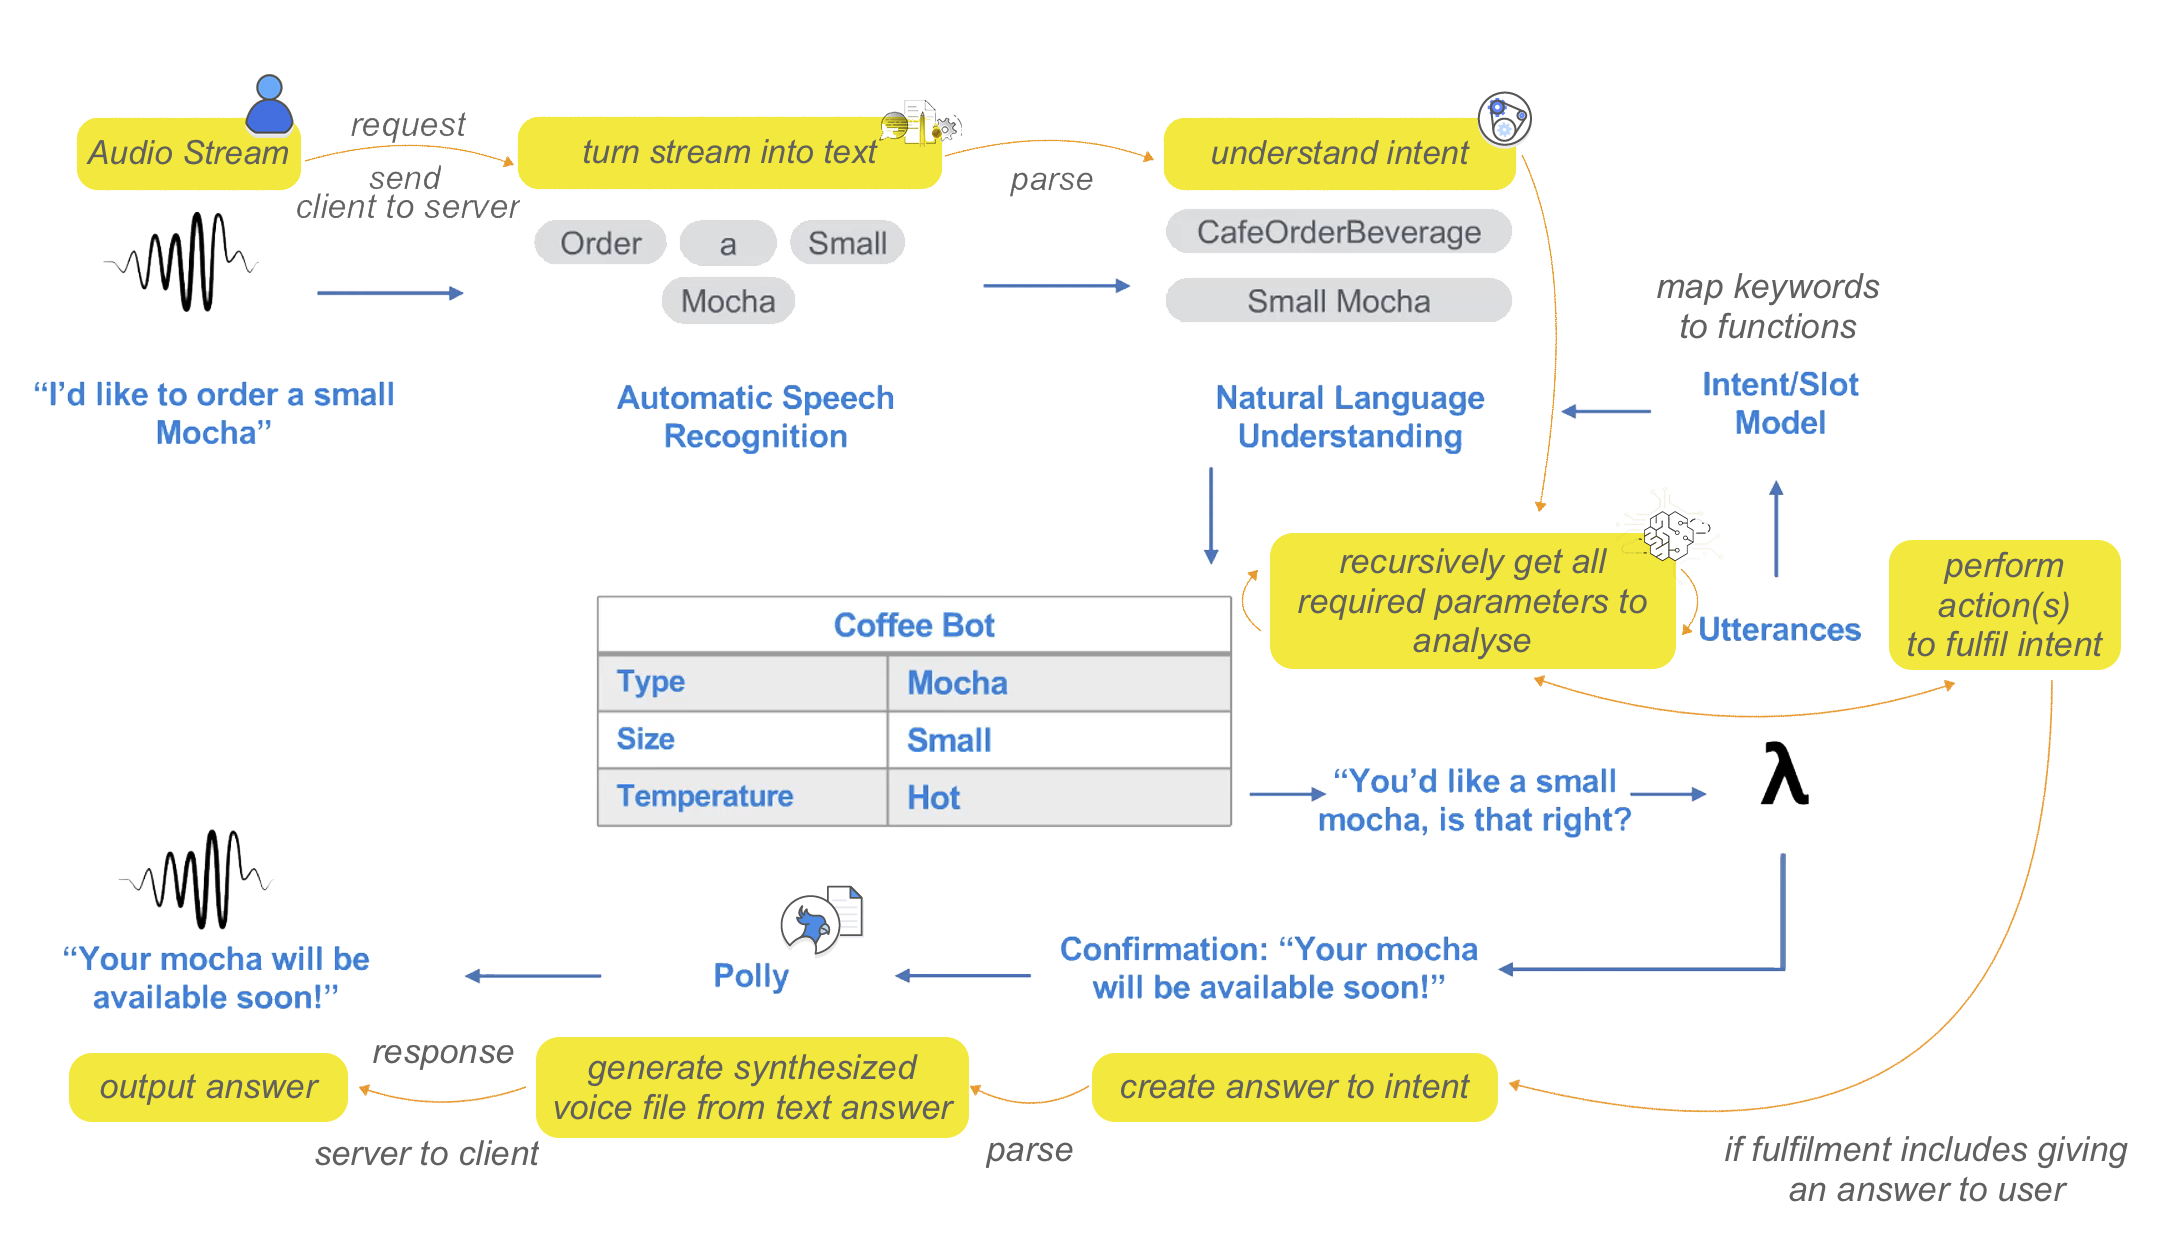
\includegraphics[width=14.8cm]{workflows/awstools.png}
\end{figure}
%
%\begin{wrapfigure}{l}{1.5cm}
%	\caption{Interaction between AWS modules in the use case of a ``Coffee Bot''}\label{lex_interactionExample}
%	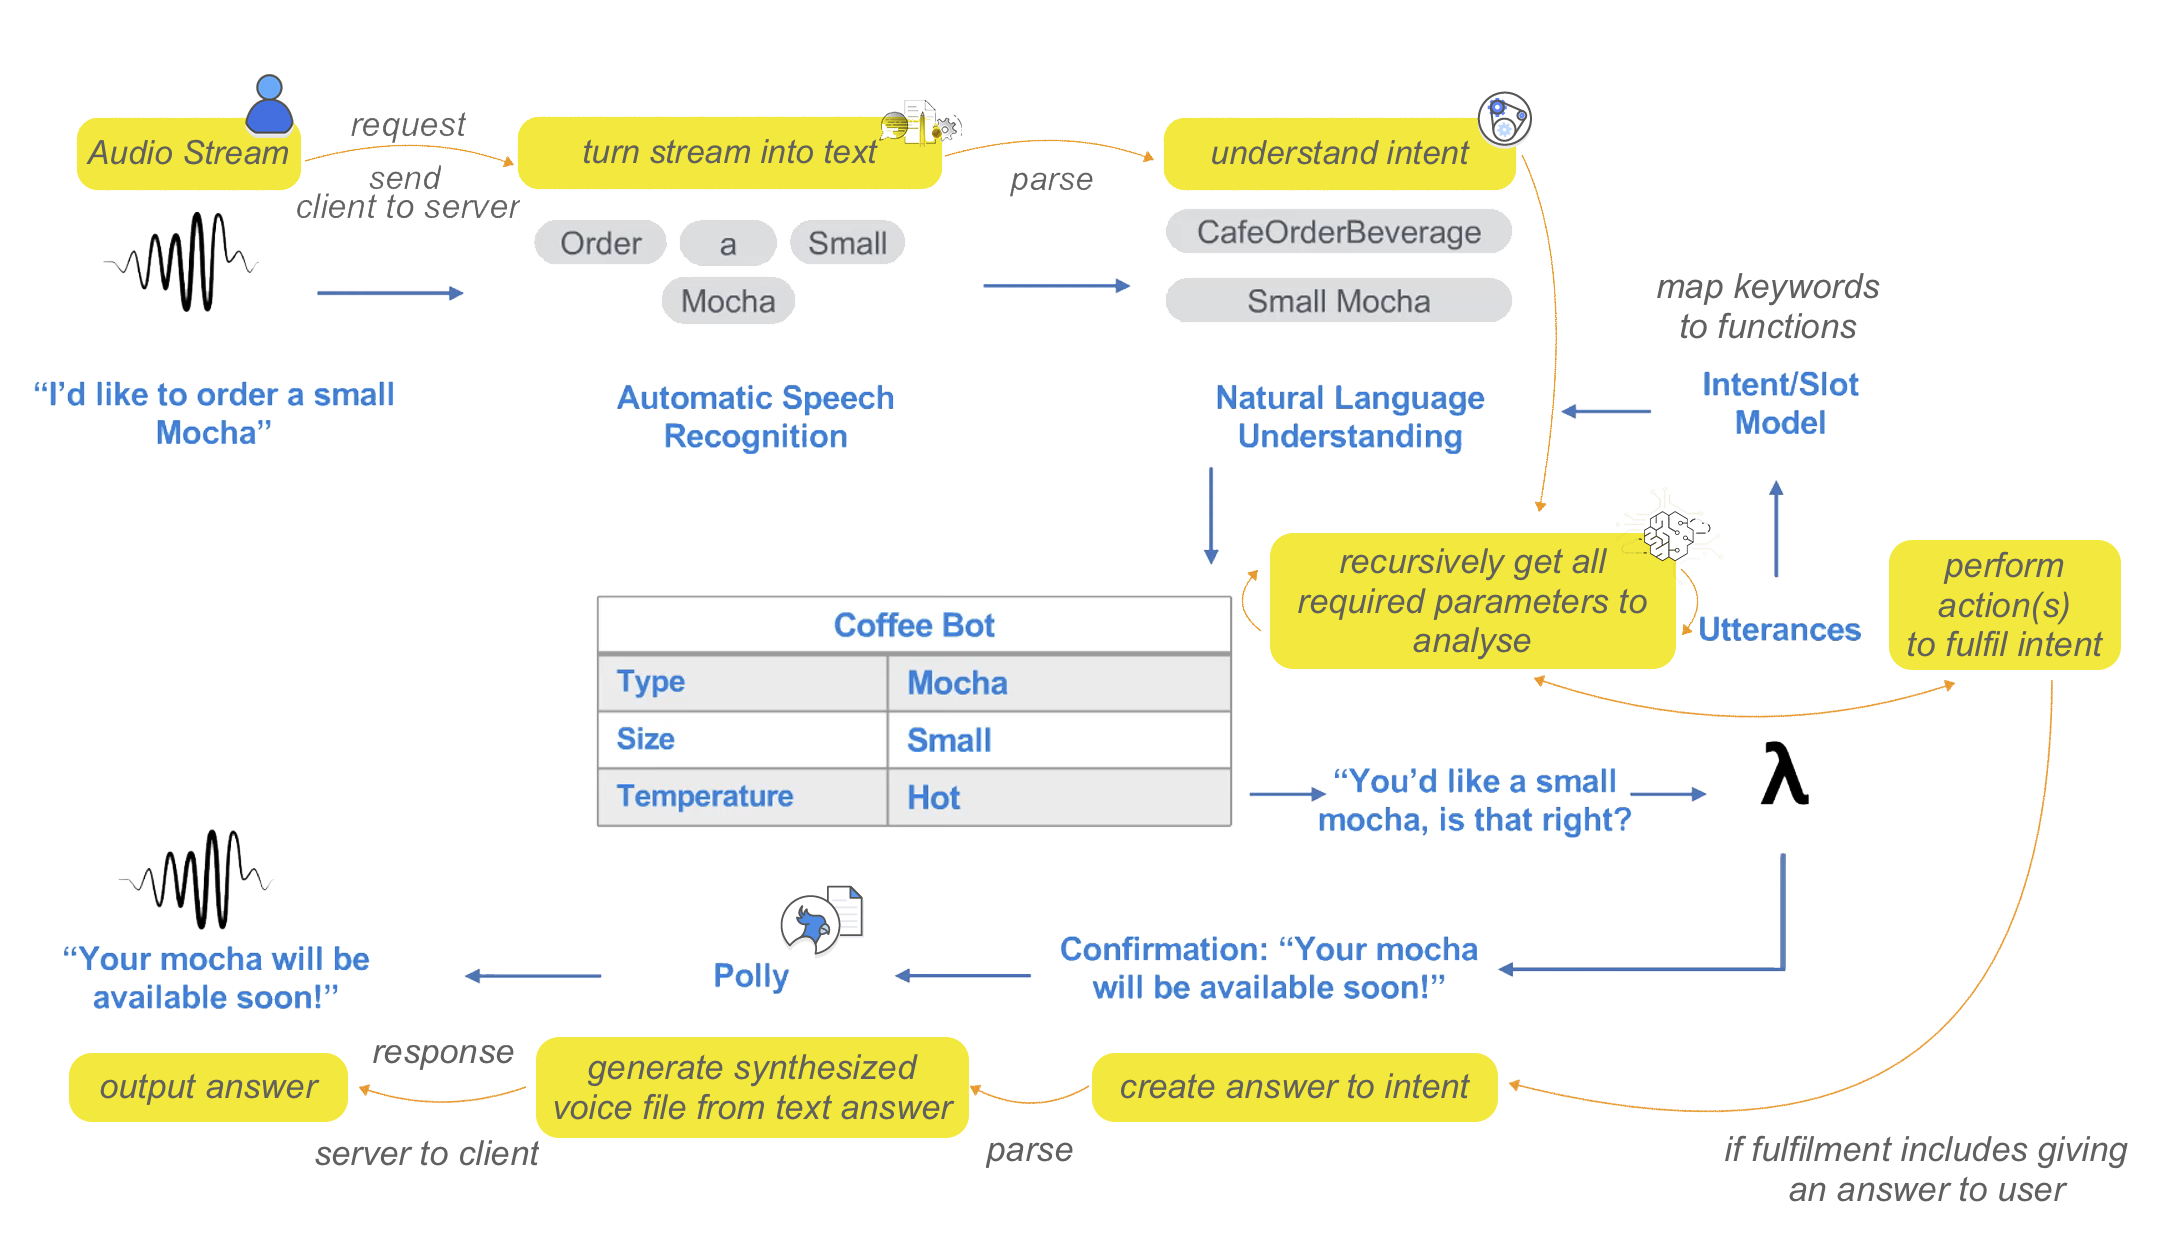
\includegraphics[width=10.5cm]{workflows/awstools.png}
%\end{wrapfigure}

putting different combinations of these and other building blocks interactively together generates the model for Alexa. In a world increasingly operated by Internet of Things (IoT), we describe a possible interaction in the example here for a use case of a hypothetical chatbot that operates a coffee machine using some of these service modules (Figure \ref{lex_interactionExample}).  Although this graphic describes how an end user would combine these modules to set up their own chatbot, this is the same workflow that Alexa uses. Hence, with Amazon's use of its own micro-services we infer that takes advantage of these to build a whole new ecosystem putting Alexa Skill developers as producers, end-users as consumers, and the Amazon website and Alexa App as a marketplace to mediate between the products (Skills) the developers produce to their target customers (end-users, country-specific or worldwide). From a marketing perspective Amazon achieves through Alexa a vertical diversification of its product programme (where existing AWS services result in a new product expanding the value chain) while simultaneously offering an extension of its aggregator model (as opposed to a marketplace model)% https://www.feedough.com/difference-marketplace-business-model-aggregator-business-model/
 by playing as a mediator between the developer's role and that of the end-user's % (who of course could be developers, too)
% this is from what I concluded from MKT and GepIT lectures.. Prof. Küpper, Axel / Prof. Klasse-Talke, Kathrin




we can therefore describe the meta-model for Alexa similar as one %to that
of an application with several front-end and back-end components acting in a DevOps environment of cloud micro-services. Unlike in most GUI-based scenarios with an MVC design pattern \cite{wiki:mvc}, where the user uses the \mintinline{java}{controller} to manipulate the \mintinline{java}{model}, which in turn updates the \mintinline{java}{view} appearing to the user, in a VUI scenario, we need to consider that the user's paradigm to the \mintinline{java}{view} component is quite different. Before we dive into the VUI paradigm, we introduce Alexa's own implementation of it for third-party applications (i.e. Skills). These are broken down into the following elements for users and developers: %to comprise a holistic ecosystem:



	
	\subsection*{Alexa Skills Store} \textit{[for End-Users]} where someone with an Alexa-enabled device can preview a Skill before installing it, %know if they want it or not and by installing them, 
	Once installed, the own instance of Alexa becomes "smarter" by that Skill, which does not need to update from ``client side'', since it is only linked to the Amazon account and not hosted on the client (only sends requests through it).  %for now 
	This offloads the user from the overhead of % does not need to 
	thinking about updates since these happen in the back-end. 
	
	
	\subsection*{Alexa Skills Kit}~\label{ask:def} \textit{[for Developers]} Although it is hard to define it as a complete SDK for Alexa and it is still in a continuous expansion phase, it is responsible for compiling the loosely coupled tools provided by AWS and others to act as an interface for the skill from a developer point of view. This fits into the rest of Amazon's scheme of focusing on interoperable micro-services that fit multiple purposes. It includes the following essentials:
	
	%Explain what the ASK SDK does
	
		\subsubsection*{Alexa (Developer) Console}~\label{ask:devconsole} This is where all the developed Skills live. It is the gateway to the front-end of the Skill or Voice service (described below). It provides a web interface for initial setup of the Skill, a structured representation of the JSON Files that include the \textsc{language (interaction) models}, the \textsc{Skill properties}, the endpoints it uses and accounts it links to. 
		Throughout this thesis, the console has undergone major interface upgrades and additions to its core functionality. Currently it is also the place where submitting the skill for publication happens and where the simulator (discussed below) lives.
		
		\subsubsection*{ASK CLI} %\lstinline|ask-cli| 
		A Command-Line Interface tool that interacts with the Alexa Console skipping the web browser. %It is still in the making but
		Although not at a stable release yet, it has numerous functions to creating, deploying and testing our Skills. %Download with 
		Available through the Node Package Manager (NPM) \footnote{
			through \lstinline|\$ npm install ask-cli| }
		
		%green because of the dollah
		
		\subsubsection*{Alexa Voice Service} %\inote{products independent from Alexa, not sure if it's worth mentioning}
		 A service for accessing cloud-based Alexa capabilities with the support of AVS APIs, hardware kits, software tools, and documentation. Through the Alexa Voice Service Amazon has simplified the creation of conversational interfaces for device makers, allowing developers to add Alexa and intelligent voice control to new products for mobile phones and cars to smart speakers and home appliances.
		 It simplifies building voice-forward products by handling complex speech recognition and natural language understanding in the cloud \footnote{\url{https://developer.amazon.com/alexa-voice-service}}


	


\section{Skill Structure}


Finally, after presenting the core stones that take part in administering the Skill, we move on to the Skill structure. Ultimately, the elements discussed above are represented in JSON files that together with the back-end of the skill make up this web-app like composition. Because of its flexible file format, Skills back-ends can be built using one of multiple runtime environments including Node.js, Java, Python, C\# and Go. 
Not coincidently, these are the same languages supported by AWS Lambda %to developed Alexa Skills. 
%can acquire access to the Skill devel

Disregarding the programming language used for development, these statically generated files are included in the code:

\begin{itemize}

\item[\mintinline{json}{skill.json}] The Skill manifest file including its publication name on the Amazon website, invocation name in each language, a description of the Skill readable by a human, author of the Skill and other properties
\inote{maybe include our sample in Appendix}

\item[\mintinline{json}{<locale>.json}] The interaction model of the respective language. It is named after the locale the file is in and includes all slots, utterances, dialogues, custom defined slot types inter alia (file structure in Table \ref{interactionModel}).

\item[\mintinline{json}{<packageFile>}] A manifest file for required dependencies (installable through NPM for instance in the case of Node or Maven in the case of Java) for installation to run the web-app in Amazon's cloud.

\end{itemize}


%\todo{remove clearpage before print}
%\clearpage

\section{Alexa Interfaces}

Briefly going over the options available to use Alexa, we present and compare the different Hardware product lines and software solutions developed by Amazon or compatible with their voice assistant in terms of usability configurations, i.e. presentation of voice and graphical interfaces.

\subsubsection*{Hardware}

The following devices are Alexa-enabled out of the box. The voice service is either accessible through voice command within the same room or an active button press on the device.

\begin{table}[htbp!]
	\caption[Alexa Devices in Comparision]{Currently Supported Alexa-Enabled Devices in Comparison}\label{alexaDeviceTable}
	\begin{tabularx}{\textwidth}{  r | l l l l  }
		
%		category
				& Speaker							& Tablet	& SmartHome	& TV	\\ \hline \hline \\
		\textit{Models}	& \shortstack[l]{Tap, Echo \\ - Dot, - Plus}     & \shortstack[l]{Echo Show \\ Kindle Fire}    & Echo Spot & FireTV Stick \\ \hline \\
		\textit{Screen}  		& No      & 7.0" 		& 2.5'' round				&  HDMI Display      \\ \hline \\
		\textit{Line Out}		& Yes      					        & \shortstack[l]{Show: Bluetooth \\ Kindle: Yes} & 	Yes & \shortstack{via HDMI \\ \textcolor{white}{text} }      \\ \hline \\
		\textit{Alexa On} 	& Voice	Command					&
		\shortstack{excl. Fire HD 10\\Button Press}
		 %\shortstack[l]{K. 7, - HD 8:  btn press \\ - HD 10: voice cmd} 
		& Voice Command & %\shortstack{Button press \\ \textcolor{white}{text} }
		Button Press
	\end{tabularx}
\end{table}

% \inote{just make a comparison table, which one has a screen, which one has which capabilities with alexa}
%Echo, Echo Dot, Tap, FireTV


%\clearpage


%then comes el software 
\subsubsection*{Software}



while the hardware models stated above are possibilities for testing, too, they do not always serve as a primary testing environment. There are sometimes more optimised ways to automate Skill testing, for instance by running scripts that would send the transcribed text in the appropriate JSON format. This is helpful for multi-turn conversations and retaining sessions, so that one does not need to repeat the full conversation until one reaches the test breakpoint.

\begin{itemize}
	
	\item[Alexa App] designed to be a control unit that operates most Alexa-enabled devices, is not an Alexa interface\footnote{yet (although this will change soon)}. However, apart from being a tool apart from Amazon's website to install Skills and manage accounts linked to Amazon (for music streaming and other related content-based services), it is a very useful tool to track the history of conversation that took place through a respective Amazon account. We use it mainly to hear what we said and see how the text was interpreted using Lex's NLU engine. It helps for checking homonyms and nuanced utterances.
	
	
	\item[EchoSim.io] ``a browser-based online community tool for developers that simulates the look and feel of an Amazon Echo'' \footnote{\url{https://echosim.io/}}. %started from a hackathon
	
	\item[Reverb] An iOS / Android app, allowing the interaction with the Alexa instance linked to an Amazon account. Perfect option to make a qualifying device Alexa-enabled \footnote{\url{https://reverb.ai}}. 
	
	\item[Alexa Simulator] Alexa's own web-based online simulator giving JSON responses and voice feedback to the requests sent and is part of the ASK. We interact with it either through voice or with JSON requests. 
	
	\item[CLI Simulator] the command-line tool of the aforementioned simulator. Accepts strings and file uploads from the CLI and returns responses to the same interface. Obviously because the Skill is a web service in the cloud, the CLI also requires an internet connection \footnote{running command \lstinline|$ ask simulate --text <inputText> --locale <inputLocale>|}.
	
\end{itemize}



%%%%%%%%%%%%%%%%%%%%%%%%%%%%%%%%%%%%%%%%%%%%%%%%%%%%%%%%%%%%%%%%%%%%%%%%%%%%%



\subsection*{Speaking with Alexa}


We end this chapter by explaining how Alexa is designed to operate from the user's point of view particularly for Skills. A full guide is available in the \textsc{ASK documentation} in multiple languages. \footnote{\t{a\t{sk}}\href{https://developer.amazon.com/docs/custom-skills/understanding-how-users-invoke-custom-skills.html}{\lstinline|/understanding-how-users-invoke-custom-skills.html|}}

A conversation starts with any of the four wake words below, followed by the launch request, then the invocation name and lastly the utterance to action. Here is an example in English.:


\[
	\underbrace{\overbrace{Alexa}^{wake \  word}}_{\shortstack[r]{Computer\\Echo\\Amazon}} %Aktivierungswort
	, \ \ \ \ 
	\underbrace{\overbrace{ask}^{launch \ action}}_{\shortstack[l]{begin, launch, load\\open, play, resume\\run, start, tell, use}}
	\ \ \ 
	\underbrace{\overbrace{<my \ Skill>}^{invocation \ name}}_{\shortstack{Citizen \ Assistant \\ Georgia Gov}}
	\ \ \
	\underbrace{\overbrace{<to \ do \ something>}^{utterance}}_{\shortstack[r]{to tell me the costs of a license transfer\\how do I get my license transferred}}
\]



%###################################################################################
%###################### Topic C             ########################################
%###################################################################################











%Durchgestrichene bzw. lokalisierte/umbennante TODOs
%Done: Move node to implementation and don’t mention that you’re using lambda until In implementation chapter k
